\documentclass{whiteboard}
\begin{document}
\begin{frame}[plain,t]
\bbcover{OBI 2013 - Nível Júnior: Fase 1}{Tomadas}{Prof. Edson Alves}{Faculdade UnB Gama}

\end{frame}
\begin{frame}[plain,t]
\vspace*{\fill}

\bbtext{A Olimpíada Internacional de Informática (IOI, no original em inglês) é a mais prestigiada competição de
programação para alunos de ensino médio; seus aproximadamente 300 competidores se reúnem em um país
diferente todo ano para os dois dias de prova da competição. Naturalmente, os competidores usam o tempo
livre para acessar a Internet, programar e jogar em seus notebooks, mas eles se depararam com um problema:
o saguão do hotel só tem uma tomada.}

\vspace{0.2in}

\bbtext{Felizmente, os quatro competidores da equipe brasileira da IOI trouxeram cada um uma régua de tomadas,
permitindo assim ligar vários notebooks em uma tomada só; eles também podem ligar uma régua em outra
para aumentar ainda mais o número de tomadas disponíveis. No entanto, como as réguas têm muitas
tomadas, eles pediram para você escrever um programa que, dado o número de tomadas em cada régua,
determina quantas tomadas podem ser disponibilizadas no saguão do hotel.}

\vspace*{\fill}
\end{frame}
\begin{frame}[plain,t]
\vspace*{\fill}

\bbbold{Entrada}

\vspace{0.2in}

\bbtext{A entrada consiste de uma linha com quatro inteiros positivos $T_1, T_2, T_3, T_4$, indicando o número de tomadas
de cada uma das quatro réguas.}

\vspace{0.2in}

\bbbold{Saída}

\vspace{0.2in}

\bbtext{Seu programa deve imprimir uma única linha contendo um único número inteiro, indicando o número máximo
de notebooks que podem ser conectados num mesmo instante.}

\vspace{0.2in}

\bbbold{Restrições}
\vspace{-0.1in}

\bbtext{
\begin{itemize}
\item $2\leq T_i\leq 6$
\end{itemize}
}

\vspace*{\fill}
\end{frame}
\begin{frame}[plain,t]
\begin{tikzpicture}
\node[draw,opacity=0] at (0, 0) {x};
\node[draw,opacity=0] at (14, 8) {x};

	\node[anchor=west] (header) at (0, 7.0) { \bbbold{Exemplo de entrada e saída} };

\end{tikzpicture}
\end{frame}
\begin{frame}[plain,t]
\begin{tikzpicture}
\node[draw,opacity=0] at (0, 0) {x};
\node[draw,opacity=0] at (14, 8) {x};

	\node[anchor=west] (header) at (0, 7.0) { \bbbold{Exemplo de entrada e saída} };


	\node[anchor=west] (line1) at (1.0, 6.0) { \bbtext{\texttt{2 4 3 2} } };

\end{tikzpicture}
\end{frame}
\begin{frame}[plain,t]
\begin{tikzpicture}
\node[draw,opacity=0] at (0, 0) {x};
\node[draw,opacity=0] at (14, 8) {x};

	\node[anchor=west] (header) at (0, 7.0) { \bbbold{Exemplo de entrada e saída} };


	\node[anchor=west] (line1) at (1.0, 6.0) { \bbtext{\texttt{2 4 3 2} } };


	\draw[->,color=BBViolet] (1.25, 5.0) to  (1.25, 5.75);

	\node[] (r) at (1.25, 4.75) { \footnotesize \bbcomment{\# de tomadas} };

	\node[] (s) at (1.25, 4.25) { \footnotesize \bbcomment{na régua $1$} };


\end{tikzpicture}
\end{frame}
\begin{frame}[plain,t]
\begin{tikzpicture}
\node[draw,opacity=0] at (0, 0) {x};
\node[draw,opacity=0] at (14, 8) {x};

	\node[anchor=west] (header) at (0, 7.0) { \bbbold{Exemplo de entrada e saída} };


	\node[anchor=west] (line1) at (1.0, 6.0) { \bbtext{\texttt{2 4 3 2} } };


	\draw[->,color=BBViolet] (1.65, 5.0) to  (1.65, 5.75);

	\node[] (r) at (1.65, 4.75) { \footnotesize \bbcomment{\# de tomadas} };

	\node[] (s) at (1.65, 4.25) { \footnotesize \bbcomment{na régua $2$} };





\end{tikzpicture}
\end{frame}
\begin{frame}[plain,t]
\begin{tikzpicture}
\node[draw,opacity=0] at (0, 0) {x};
\node[draw,opacity=0] at (14, 8) {x};

	\node[anchor=west] (header) at (0, 7.0) { \bbbold{Exemplo de entrada e saída} };


	\node[anchor=west] (line1) at (1.0, 6.0) { \bbtext{\texttt{2 4 3 2} } };


	\draw[->,color=BBViolet] (2.05, 5.0) to  (2.05, 5.75);

	\node[] (r) at (2.05, 4.75) { \footnotesize \bbcomment{\# de tomadas} };

	\node[] (s) at (2.05, 4.25) { \footnotesize \bbcomment{na régua $3$} };







\end{tikzpicture}
\end{frame}
\begin{frame}[plain,t]
\begin{tikzpicture}
\node[draw,opacity=0] at (0, 0) {x};
\node[draw,opacity=0] at (14, 8) {x};

	\node[anchor=west] (header) at (0, 7.0) { \bbbold{Exemplo de entrada e saída} };


	\node[anchor=west] (line1) at (1.0, 6.0) { \bbtext{\texttt{2 4 3 2} } };


	\draw[->,color=BBViolet] (2.45, 5.0) to  (2.45, 5.75);

	\node[] (r) at (2.45, 4.75) { \footnotesize \bbcomment{\# de tomadas} };

	\node[] (s) at (2.45, 4.25) { \footnotesize \bbcomment{na régua $4$} };









\end{tikzpicture}
\end{frame}
\begin{frame}[plain,t]
\begin{tikzpicture}
\node[draw,opacity=0] at (0, 0) {x};
\node[draw,opacity=0] at (14, 8) {x};

	\node[anchor=west] (header) at (0, 7.0) { \bbbold{Exemplo de entrada e saída} };


	\node[anchor=west] (line1) at (1.0, 6.0) { \bbtext{\texttt{2 4 3 2} } };















	\draw[thick,rounded corners] (1, 3.5) rectangle (2, 5);

	\draw[fill=yellow!50!white,thick] (1.5, 4.25) circle (0.35);

	\draw[ultra thick,rounded corners] (1.375, 4.1) to (1.375, 4.4);

	\draw[ultra thick,rounded corners] (1.625, 4.1) to (1.625, 4.4);

\end{tikzpicture}
\end{frame}
\begin{frame}[plain,t]
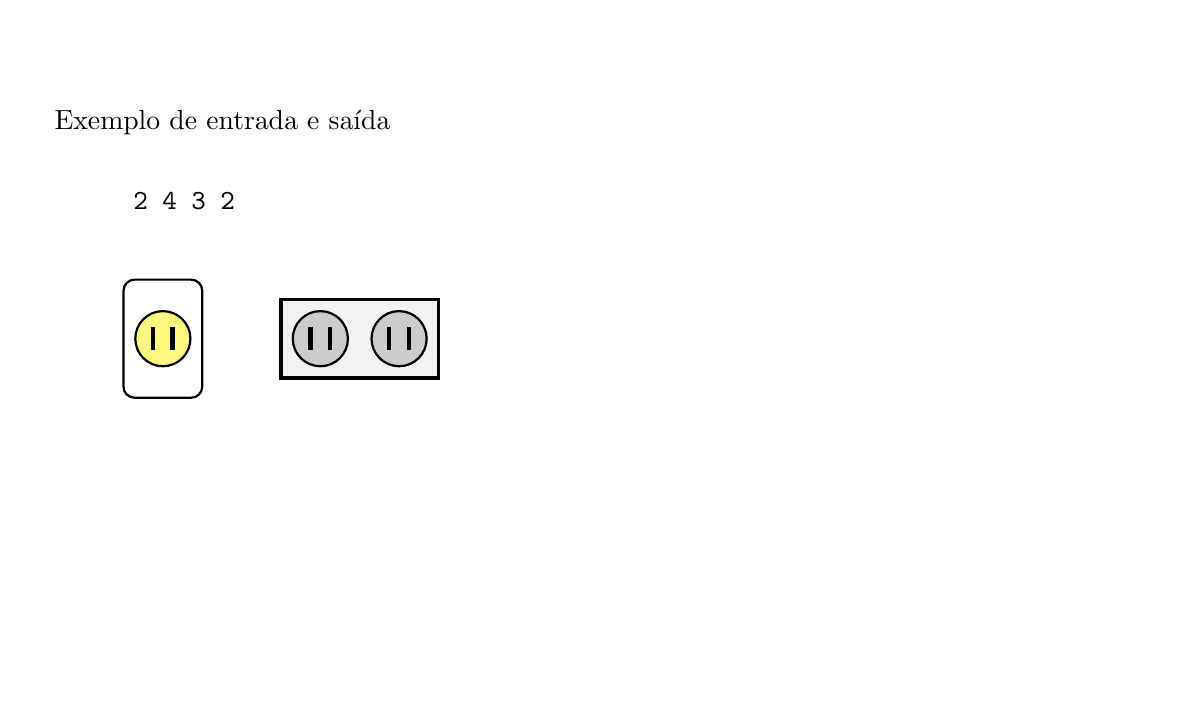
\begin{tikzpicture}
\node[draw,opacity=0] at (0, 0) {x};
\node[draw,opacity=0] at (14, 8) {x};

	\node[anchor=west] (header) at (0, 7.0) { \bbbold{Exemplo de entrada e saída} };


	\node[anchor=west] (line1) at (1.0, 6.0) { \bbtext{\texttt{2 4 3 2} } };















	\draw[thick,rounded corners] (1, 3.5) rectangle (2, 5);

	\draw[fill=yellow!50!white,thick] (1.5, 4.25) circle (0.35);

	\draw[ultra thick,rounded corners] (1.375, 4.1) to (1.375, 4.4);

	\draw[ultra thick,rounded corners] (1.625, 4.1) to (1.625, 4.4);


	\draw[fill=gray!10!white,very thick] (3, 3.75) rectangle (5, 4.75);

	\draw[fill=gray!40!white,thick] (3.5, 4.25) circle (0.35);

	\draw[ultra thick,rounded corners] (3.375, 4.1) to (3.375, 4.4);

	\draw[ultra thick,rounded corners] (3.625, 4.1) to (3.625, 4.4);

	\draw[fill=gray!40!white,thick] (4.5, 4.25) circle (0.35);

	\draw[ultra thick,rounded corners] (4.375, 4.1) to (4.375, 4.4);

	\draw[ultra thick,rounded corners] (4.625, 4.1) to (4.625, 4.4);

\end{tikzpicture}
\end{frame}
\begin{frame}[plain,t]
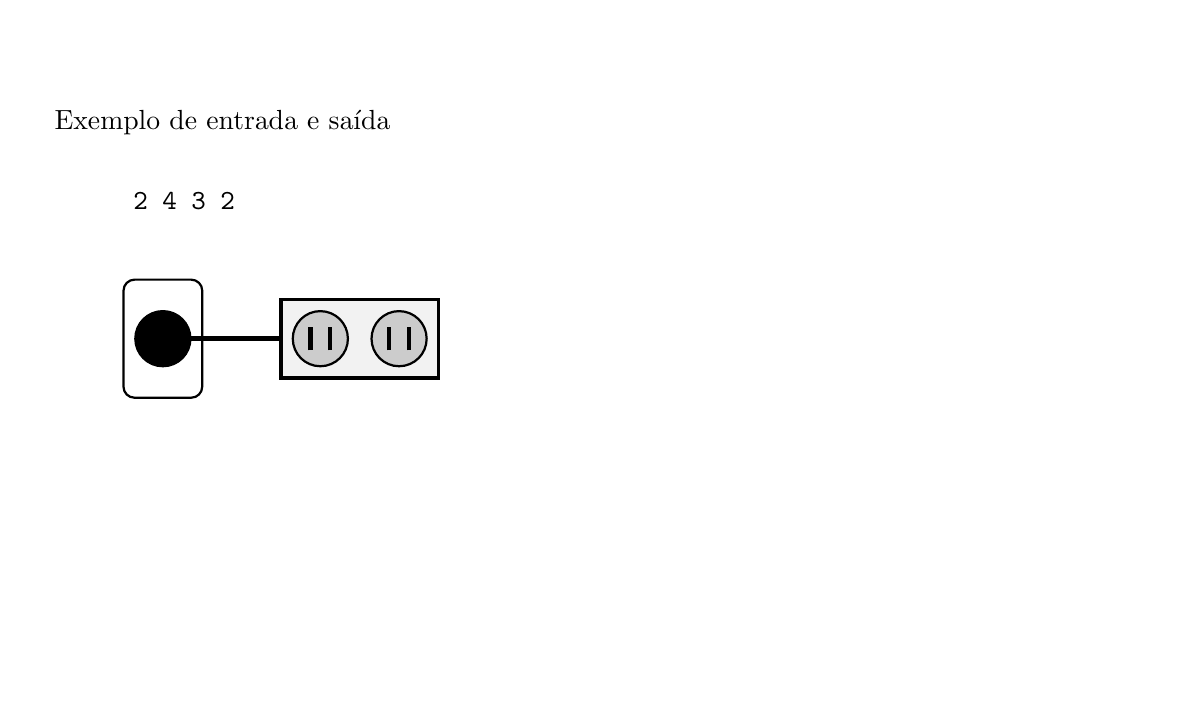
\begin{tikzpicture}
\node[draw,opacity=0] at (0, 0) {x};
\node[draw,opacity=0] at (14, 8) {x};

	\node[anchor=west] (header) at (0, 7.0) { \bbbold{Exemplo de entrada e saída} };


	\node[anchor=west] (line1) at (1.0, 6.0) { \bbtext{\texttt{2 4 3 2} } };















	\draw[thick,rounded corners] (1, 3.5) rectangle (2, 5);

	\draw[fill=black,thick] (1.5, 4.25) circle (0.35);

	\draw[ultra thick,rounded corners] (1.375, 4.1) to (1.375, 4.4);

	\draw[ultra thick,rounded corners] (1.625, 4.1) to (1.625, 4.4);


	\draw[fill=gray!10!white,very thick] (3, 3.75) rectangle (5, 4.75);

	\draw[fill=gray!40!white,thick] (3.5, 4.25) circle (0.35);

	\draw[ultra thick,rounded corners] (3.375, 4.1) to (3.375, 4.4);

	\draw[ultra thick,rounded corners] (3.625, 4.1) to (3.625, 4.4);

	\draw[fill=gray!40!white,thick] (4.5, 4.25) circle (0.35);

	\draw[ultra thick,rounded corners] (4.375, 4.1) to (4.375, 4.4);

	\draw[ultra thick,rounded corners] (4.625, 4.1) to (4.625, 4.4);


	\draw[ultra thick] (3, 4.25) to (1.8, 4.25);


\end{tikzpicture}
\end{frame}
\begin{frame}[plain,t]
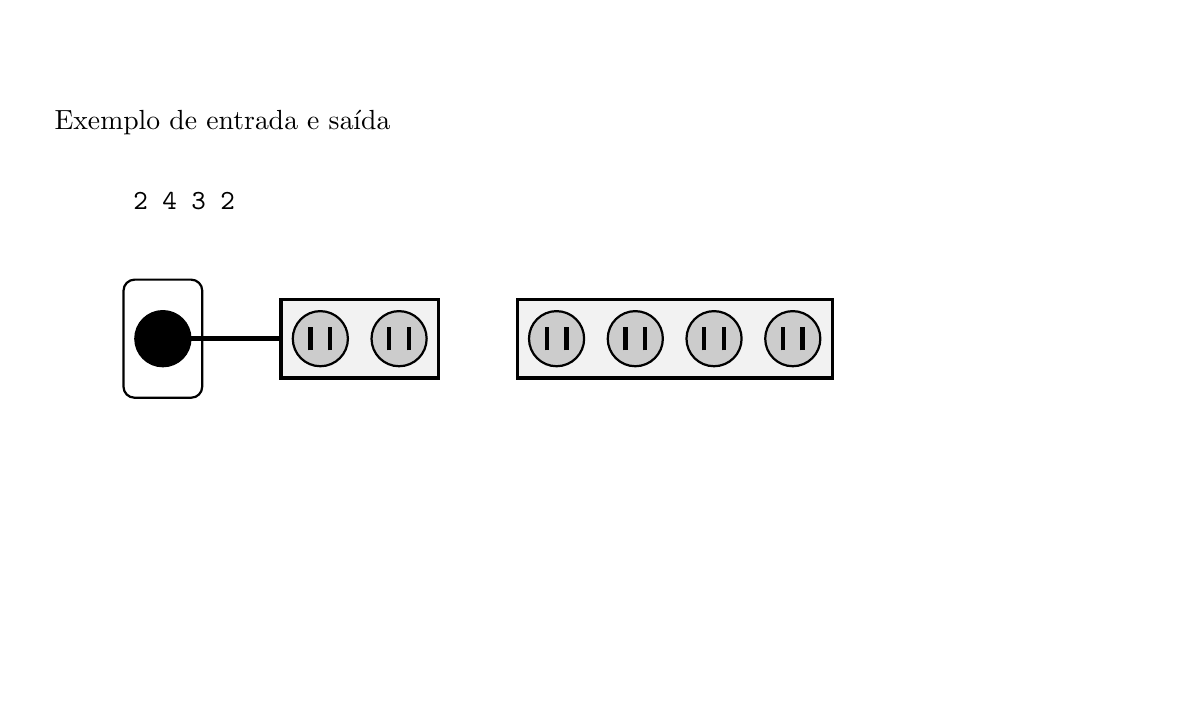
\begin{tikzpicture}
\node[draw,opacity=0] at (0, 0) {x};
\node[draw,opacity=0] at (14, 8) {x};

	\node[anchor=west] (header) at (0, 7.0) { \bbbold{Exemplo de entrada e saída} };


	\node[anchor=west] (line1) at (1.0, 6.0) { \bbtext{\texttt{2 4 3 2} } };















	\draw[thick,rounded corners] (1, 3.5) rectangle (2, 5);

	\draw[fill=black,thick] (1.5, 4.25) circle (0.35);

	\draw[ultra thick,rounded corners] (1.375, 4.1) to (1.375, 4.4);

	\draw[ultra thick,rounded corners] (1.625, 4.1) to (1.625, 4.4);


	\draw[fill=gray!10!white,very thick] (3, 3.75) rectangle (5, 4.75);

	\draw[fill=gray!40!white,thick] (3.5, 4.25) circle (0.35);

	\draw[ultra thick,rounded corners] (3.375, 4.1) to (3.375, 4.4);

	\draw[ultra thick,rounded corners] (3.625, 4.1) to (3.625, 4.4);

	\draw[fill=gray!40!white,thick] (4.5, 4.25) circle (0.35);

	\draw[ultra thick,rounded corners] (4.375, 4.1) to (4.375, 4.4);

	\draw[ultra thick,rounded corners] (4.625, 4.1) to (4.625, 4.4);


	\draw[ultra thick] (3, 4.25) to (1.8, 4.25);



	\draw[fill=gray!10!white,very thick] (6, 3.75) rectangle (10, 4.75);

	\draw[fill=gray!40!white,thick] (6.5, 4.25) circle (0.35);

	\draw[ultra thick,rounded corners] (6.375, 4.1) to (6.375, 4.4);

	\draw[ultra thick,rounded corners] (6.625, 4.1) to (6.625, 4.4);

	\draw[fill=gray!40!white,thick] (7.5, 4.25) circle (0.35);

	\draw[ultra thick,rounded corners] (7.375, 4.1) to (7.375, 4.4);

	\draw[ultra thick,rounded corners] (7.625, 4.1) to (7.625, 4.4);

	\draw[fill=gray!40!white,thick] (8.5, 4.25) circle (0.35);

	\draw[ultra thick,rounded corners] (8.375, 4.1) to (8.375, 4.4);

	\draw[ultra thick,rounded corners] (8.625, 4.1) to (8.625, 4.4);

	\draw[fill=gray!40!white,thick] (9.5, 4.25) circle (0.35);

	\draw[ultra thick,rounded corners] (9.375, 4.1) to (9.375, 4.4);

	\draw[ultra thick,rounded corners] (9.625, 4.1) to (9.625, 4.4);

\end{tikzpicture}
\end{frame}
\begin{frame}[plain,t]
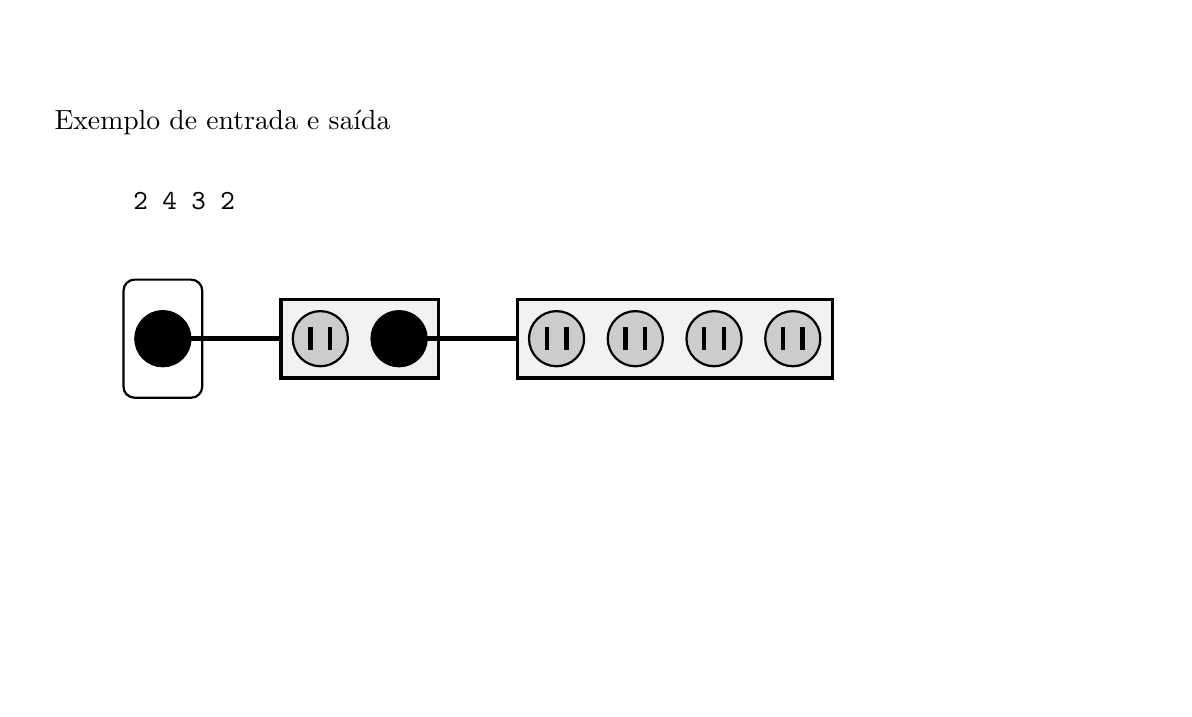
\begin{tikzpicture}
\node[draw,opacity=0] at (0, 0) {x};
\node[draw,opacity=0] at (14, 8) {x};

	\node[anchor=west] (header) at (0, 7.0) { \bbbold{Exemplo de entrada e saída} };


	\node[anchor=west] (line1) at (1.0, 6.0) { \bbtext{\texttt{2 4 3 2} } };















	\draw[thick,rounded corners] (1, 3.5) rectangle (2, 5);

	\draw[fill=black,thick] (1.5, 4.25) circle (0.35);

	\draw[ultra thick,rounded corners] (1.375, 4.1) to (1.375, 4.4);

	\draw[ultra thick,rounded corners] (1.625, 4.1) to (1.625, 4.4);


	\draw[fill=gray!10!white,very thick] (3, 3.75) rectangle (5, 4.75);

	\draw[fill=gray!40!white,thick] (3.5, 4.25) circle (0.35);

	\draw[ultra thick,rounded corners] (3.375, 4.1) to (3.375, 4.4);

	\draw[ultra thick,rounded corners] (3.625, 4.1) to (3.625, 4.4);

	\draw[fill=black,thick] (4.5, 4.25) circle (0.35);

	\draw[ultra thick,rounded corners] (4.375, 4.1) to (4.375, 4.4);

	\draw[ultra thick,rounded corners] (4.625, 4.1) to (4.625, 4.4);


	\draw[ultra thick] (3, 4.25) to (1.8, 4.25);



	\draw[fill=gray!10!white,very thick] (6, 3.75) rectangle (10, 4.75);

	\draw[fill=gray!40!white,thick] (6.5, 4.25) circle (0.35);

	\draw[ultra thick,rounded corners] (6.375, 4.1) to (6.375, 4.4);

	\draw[ultra thick,rounded corners] (6.625, 4.1) to (6.625, 4.4);

	\draw[fill=gray!40!white,thick] (7.5, 4.25) circle (0.35);

	\draw[ultra thick,rounded corners] (7.375, 4.1) to (7.375, 4.4);

	\draw[ultra thick,rounded corners] (7.625, 4.1) to (7.625, 4.4);

	\draw[fill=gray!40!white,thick] (8.5, 4.25) circle (0.35);

	\draw[ultra thick,rounded corners] (8.375, 4.1) to (8.375, 4.4);

	\draw[ultra thick,rounded corners] (8.625, 4.1) to (8.625, 4.4);

	\draw[fill=gray!40!white,thick] (9.5, 4.25) circle (0.35);

	\draw[ultra thick,rounded corners] (9.375, 4.1) to (9.375, 4.4);

	\draw[ultra thick,rounded corners] (9.625, 4.1) to (9.625, 4.4);


	\draw[ultra thick] (6, 4.25) to (4.8, 4.25);


\end{tikzpicture}
\end{frame}
\begin{frame}[plain,t]
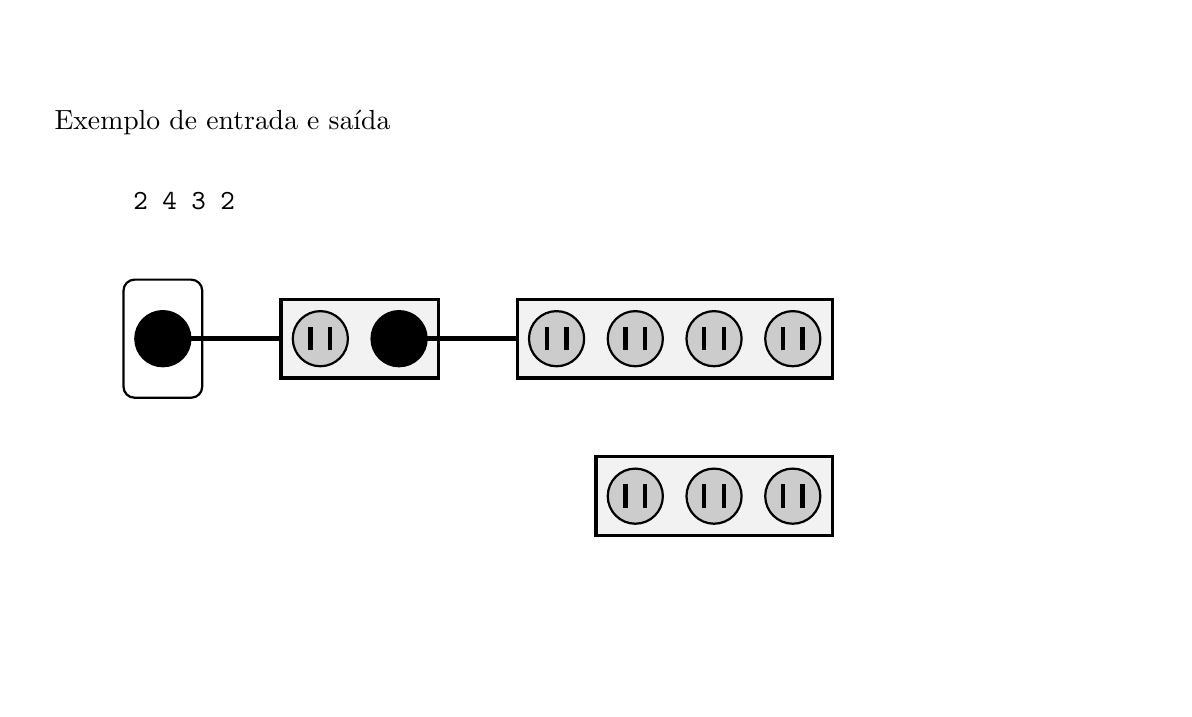
\begin{tikzpicture}
\node[draw,opacity=0] at (0, 0) {x};
\node[draw,opacity=0] at (14, 8) {x};

	\node[anchor=west] (header) at (0, 7.0) { \bbbold{Exemplo de entrada e saída} };


	\node[anchor=west] (line1) at (1.0, 6.0) { \bbtext{\texttt{2 4 3 2} } };















	\draw[thick,rounded corners] (1, 3.5) rectangle (2, 5);

	\draw[fill=black,thick] (1.5, 4.25) circle (0.35);

	\draw[ultra thick,rounded corners] (1.375, 4.1) to (1.375, 4.4);

	\draw[ultra thick,rounded corners] (1.625, 4.1) to (1.625, 4.4);


	\draw[fill=gray!10!white,very thick] (3, 3.75) rectangle (5, 4.75);

	\draw[fill=gray!40!white,thick] (3.5, 4.25) circle (0.35);

	\draw[ultra thick,rounded corners] (3.375, 4.1) to (3.375, 4.4);

	\draw[ultra thick,rounded corners] (3.625, 4.1) to (3.625, 4.4);

	\draw[fill=black,thick] (4.5, 4.25) circle (0.35);

	\draw[ultra thick,rounded corners] (4.375, 4.1) to (4.375, 4.4);

	\draw[ultra thick,rounded corners] (4.625, 4.1) to (4.625, 4.4);


	\draw[ultra thick] (3, 4.25) to (1.8, 4.25);



	\draw[fill=gray!10!white,very thick] (6, 3.75) rectangle (10, 4.75);

	\draw[fill=gray!40!white,thick] (6.5, 4.25) circle (0.35);

	\draw[ultra thick,rounded corners] (6.375, 4.1) to (6.375, 4.4);

	\draw[ultra thick,rounded corners] (6.625, 4.1) to (6.625, 4.4);

	\draw[fill=gray!40!white,thick] (7.5, 4.25) circle (0.35);

	\draw[ultra thick,rounded corners] (7.375, 4.1) to (7.375, 4.4);

	\draw[ultra thick,rounded corners] (7.625, 4.1) to (7.625, 4.4);

	\draw[fill=gray!40!white,thick] (8.5, 4.25) circle (0.35);

	\draw[ultra thick,rounded corners] (8.375, 4.1) to (8.375, 4.4);

	\draw[ultra thick,rounded corners] (8.625, 4.1) to (8.625, 4.4);

	\draw[fill=gray!40!white,thick] (9.5, 4.25) circle (0.35);

	\draw[ultra thick,rounded corners] (9.375, 4.1) to (9.375, 4.4);

	\draw[ultra thick,rounded corners] (9.625, 4.1) to (9.625, 4.4);


	\draw[ultra thick] (6, 4.25) to (4.8, 4.25);



	\draw[fill=gray!10!white,very thick] (7, 1.75) rectangle (10, 2.75);

	\draw[fill=gray!40!white,thick] (9.5, 2.25) circle (0.35);

	\draw[ultra thick,rounded corners] (9.375, 2.1) to (9.375, 2.4);

	\draw[ultra thick,rounded corners] (9.625, 2.1) to (9.625, 2.4);

	\draw[fill=gray!40!white,thick] (8.5, 2.25) circle (0.35);

	\draw[ultra thick,rounded corners] (8.375, 2.1) to (8.375, 2.4);

	\draw[ultra thick,rounded corners] (8.625, 2.1) to (8.625, 2.4);

	\draw[fill=gray!40!white,thick] (7.5, 2.25) circle (0.35);

	\draw[ultra thick,rounded corners] (7.375, 2.1) to (7.375, 2.4);

	\draw[ultra thick,rounded corners] (7.625, 2.1) to (7.625, 2.4);

\end{tikzpicture}
\end{frame}
\begin{frame}[plain,t]
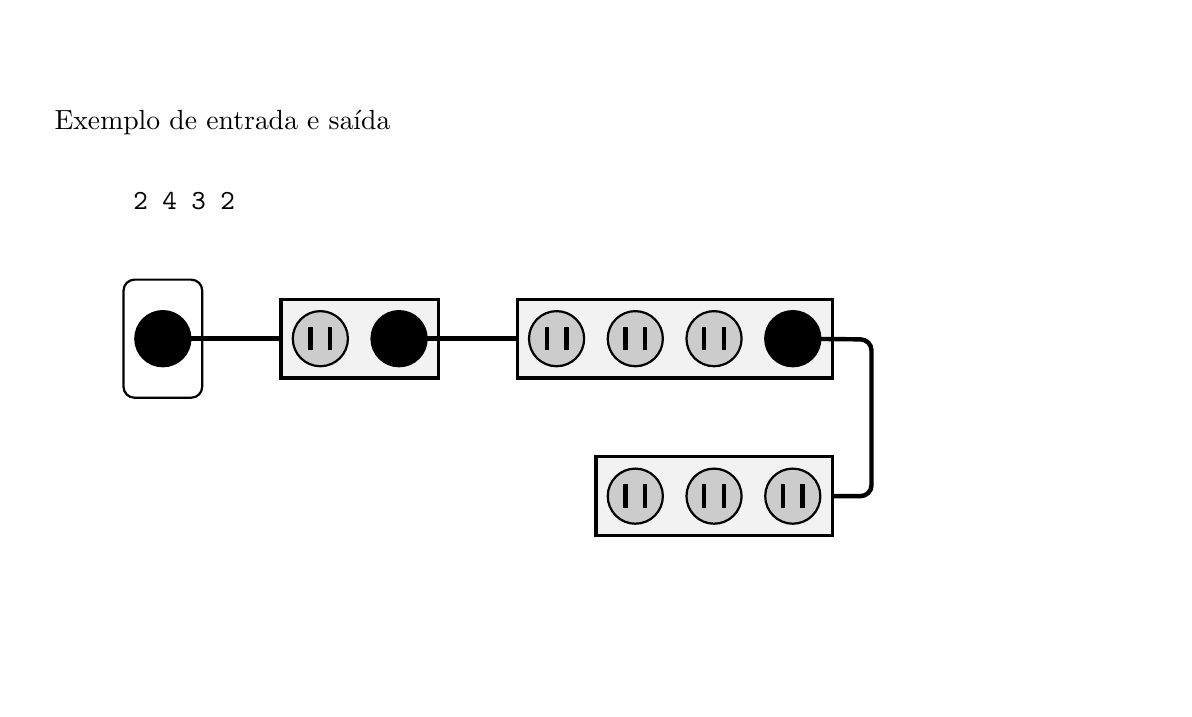
\begin{tikzpicture}
\node[draw,opacity=0] at (0, 0) {x};
\node[draw,opacity=0] at (14, 8) {x};

	\node[anchor=west] (header) at (0, 7.0) { \bbbold{Exemplo de entrada e saída} };


	\node[anchor=west] (line1) at (1.0, 6.0) { \bbtext{\texttt{2 4 3 2} } };















	\draw[thick,rounded corners] (1, 3.5) rectangle (2, 5);

	\draw[fill=black,thick] (1.5, 4.25) circle (0.35);

	\draw[ultra thick,rounded corners] (1.375, 4.1) to (1.375, 4.4);

	\draw[ultra thick,rounded corners] (1.625, 4.1) to (1.625, 4.4);


	\draw[fill=gray!10!white,very thick] (3, 3.75) rectangle (5, 4.75);

	\draw[fill=gray!40!white,thick] (3.5, 4.25) circle (0.35);

	\draw[ultra thick,rounded corners] (3.375, 4.1) to (3.375, 4.4);

	\draw[ultra thick,rounded corners] (3.625, 4.1) to (3.625, 4.4);

	\draw[fill=black,thick] (4.5, 4.25) circle (0.35);

	\draw[ultra thick,rounded corners] (4.375, 4.1) to (4.375, 4.4);

	\draw[ultra thick,rounded corners] (4.625, 4.1) to (4.625, 4.4);


	\draw[ultra thick] (3, 4.25) to (1.8, 4.25);



	\draw[fill=gray!10!white,very thick] (6, 3.75) rectangle (10, 4.75);

	\draw[fill=gray!40!white,thick] (6.5, 4.25) circle (0.35);

	\draw[ultra thick,rounded corners] (6.375, 4.1) to (6.375, 4.4);

	\draw[ultra thick,rounded corners] (6.625, 4.1) to (6.625, 4.4);

	\draw[fill=gray!40!white,thick] (7.5, 4.25) circle (0.35);

	\draw[ultra thick,rounded corners] (7.375, 4.1) to (7.375, 4.4);

	\draw[ultra thick,rounded corners] (7.625, 4.1) to (7.625, 4.4);

	\draw[fill=gray!40!white,thick] (8.5, 4.25) circle (0.35);

	\draw[ultra thick,rounded corners] (8.375, 4.1) to (8.375, 4.4);

	\draw[ultra thick,rounded corners] (8.625, 4.1) to (8.625, 4.4);

	\draw[fill=black,thick] (9.5, 4.25) circle (0.35);

	\draw[ultra thick,rounded corners] (9.375, 4.1) to (9.375, 4.4);

	\draw[ultra thick,rounded corners] (9.625, 4.1) to (9.625, 4.4);


	\draw[ultra thick] (6, 4.25) to (4.8, 4.25);



	\draw[fill=gray!10!white,very thick] (7, 1.75) rectangle (10, 2.75);

	\draw[fill=gray!40!white,thick] (9.5, 2.25) circle (0.35);

	\draw[ultra thick,rounded corners] (9.375, 2.1) to (9.375, 2.4);

	\draw[ultra thick,rounded corners] (9.625, 2.1) to (9.625, 2.4);

	\draw[fill=gray!40!white,thick] (8.5, 2.25) circle (0.35);

	\draw[ultra thick,rounded corners] (8.375, 2.1) to (8.375, 2.4);

	\draw[ultra thick,rounded corners] (8.625, 2.1) to (8.625, 2.4);

	\draw[fill=gray!40!white,thick] (7.5, 2.25) circle (0.35);

	\draw[ultra thick,rounded corners] (7.375, 2.1) to (7.375, 2.4);

	\draw[ultra thick,rounded corners] (7.625, 2.1) to (7.625, 2.4);


	\draw[ultra thick,rounded corners] (10, 2.25) to (10.5, 2.25) to (10.5, 4.24) to (9.5, 4.25);


\end{tikzpicture}
\end{frame}
\begin{frame}[plain,t]
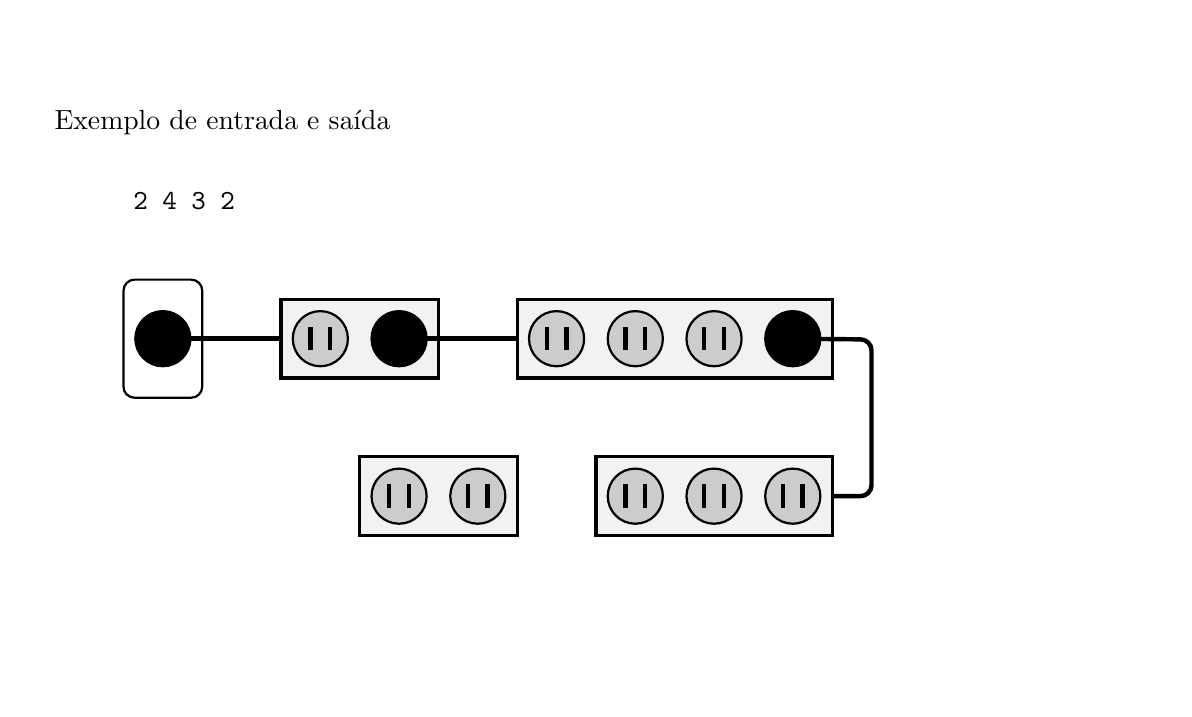
\begin{tikzpicture}
\node[draw,opacity=0] at (0, 0) {x};
\node[draw,opacity=0] at (14, 8) {x};

	\node[anchor=west] (header) at (0, 7.0) { \bbbold{Exemplo de entrada e saída} };


	\node[anchor=west] (line1) at (1.0, 6.0) { \bbtext{\texttt{2 4 3 2} } };















	\draw[thick,rounded corners] (1, 3.5) rectangle (2, 5);

	\draw[fill=black,thick] (1.5, 4.25) circle (0.35);

	\draw[ultra thick,rounded corners] (1.375, 4.1) to (1.375, 4.4);

	\draw[ultra thick,rounded corners] (1.625, 4.1) to (1.625, 4.4);


	\draw[fill=gray!10!white,very thick] (3, 3.75) rectangle (5, 4.75);

	\draw[fill=gray!40!white,thick] (3.5, 4.25) circle (0.35);

	\draw[ultra thick,rounded corners] (3.375, 4.1) to (3.375, 4.4);

	\draw[ultra thick,rounded corners] (3.625, 4.1) to (3.625, 4.4);

	\draw[fill=black,thick] (4.5, 4.25) circle (0.35);

	\draw[ultra thick,rounded corners] (4.375, 4.1) to (4.375, 4.4);

	\draw[ultra thick,rounded corners] (4.625, 4.1) to (4.625, 4.4);


	\draw[ultra thick] (3, 4.25) to (1.8, 4.25);



	\draw[fill=gray!10!white,very thick] (6, 3.75) rectangle (10, 4.75);

	\draw[fill=gray!40!white,thick] (6.5, 4.25) circle (0.35);

	\draw[ultra thick,rounded corners] (6.375, 4.1) to (6.375, 4.4);

	\draw[ultra thick,rounded corners] (6.625, 4.1) to (6.625, 4.4);

	\draw[fill=gray!40!white,thick] (7.5, 4.25) circle (0.35);

	\draw[ultra thick,rounded corners] (7.375, 4.1) to (7.375, 4.4);

	\draw[ultra thick,rounded corners] (7.625, 4.1) to (7.625, 4.4);

	\draw[fill=gray!40!white,thick] (8.5, 4.25) circle (0.35);

	\draw[ultra thick,rounded corners] (8.375, 4.1) to (8.375, 4.4);

	\draw[ultra thick,rounded corners] (8.625, 4.1) to (8.625, 4.4);

	\draw[fill=black,thick] (9.5, 4.25) circle (0.35);

	\draw[ultra thick,rounded corners] (9.375, 4.1) to (9.375, 4.4);

	\draw[ultra thick,rounded corners] (9.625, 4.1) to (9.625, 4.4);


	\draw[ultra thick] (6, 4.25) to (4.8, 4.25);



	\draw[fill=gray!10!white,very thick] (7, 1.75) rectangle (10, 2.75);

	\draw[fill=gray!40!white,thick] (9.5, 2.25) circle (0.35);

	\draw[ultra thick,rounded corners] (9.375, 2.1) to (9.375, 2.4);

	\draw[ultra thick,rounded corners] (9.625, 2.1) to (9.625, 2.4);

	\draw[fill=gray!40!white,thick] (8.5, 2.25) circle (0.35);

	\draw[ultra thick,rounded corners] (8.375, 2.1) to (8.375, 2.4);

	\draw[ultra thick,rounded corners] (8.625, 2.1) to (8.625, 2.4);

	\draw[fill=gray!40!white,thick] (7.5, 2.25) circle (0.35);

	\draw[ultra thick,rounded corners] (7.375, 2.1) to (7.375, 2.4);

	\draw[ultra thick,rounded corners] (7.625, 2.1) to (7.625, 2.4);


	\draw[ultra thick,rounded corners] (10, 2.25) to (10.5, 2.25) to (10.5, 4.24) to (9.5, 4.25);



	\draw[fill=gray!10!white,very thick] (4, 1.75) rectangle (6, 2.75);

	\draw[fill=gray!40!white,thick] (5.5, 2.25) circle (0.35);

	\draw[ultra thick,rounded corners] (5.375, 2.1) to (5.375, 2.4);

	\draw[ultra thick,rounded corners] (5.625, 2.1) to (5.625, 2.4);

	\draw[fill=gray!40!white,thick] (4.5, 2.25) circle (0.35);

	\draw[ultra thick,rounded corners] (4.375, 2.1) to (4.375, 2.4);

	\draw[ultra thick,rounded corners] (4.625, 2.1) to (4.625, 2.4);

\end{tikzpicture}
\end{frame}
\begin{frame}[plain,t]
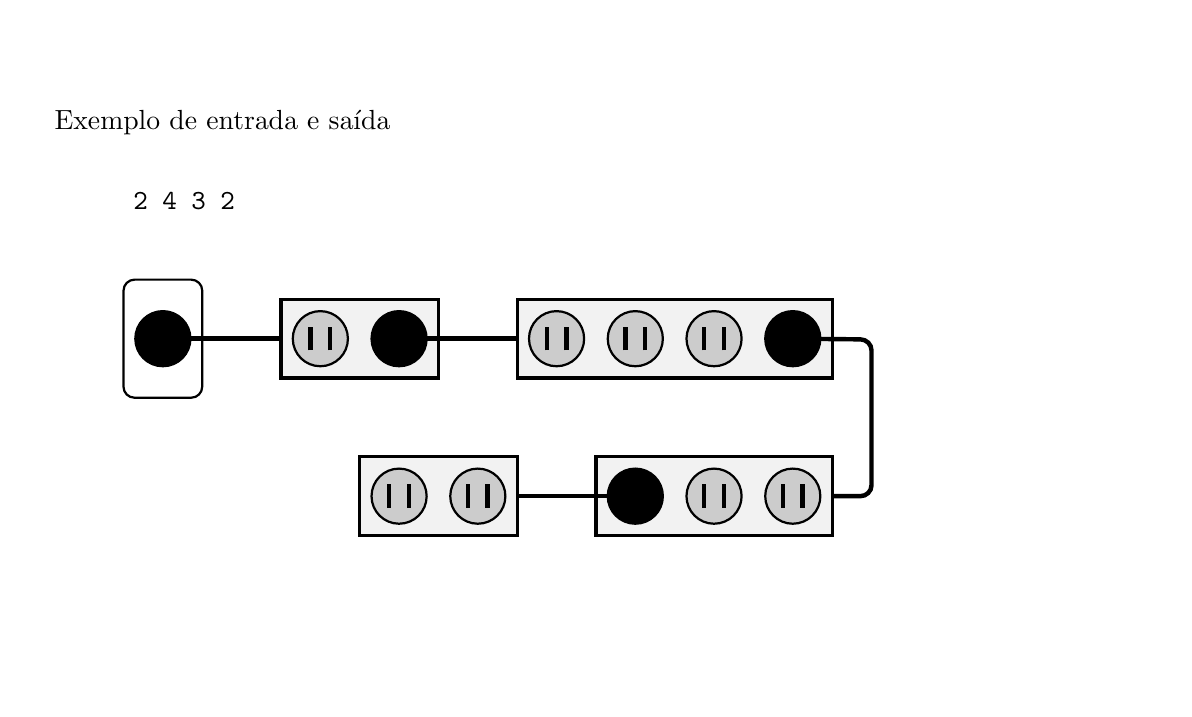
\begin{tikzpicture}
\node[draw,opacity=0] at (0, 0) {x};
\node[draw,opacity=0] at (14, 8) {x};

	\node[anchor=west] (header) at (0, 7.0) { \bbbold{Exemplo de entrada e saída} };


	\node[anchor=west] (line1) at (1.0, 6.0) { \bbtext{\texttt{2 4 3 2} } };















	\draw[thick,rounded corners] (1, 3.5) rectangle (2, 5);

	\draw[fill=black,thick] (1.5, 4.25) circle (0.35);

	\draw[ultra thick,rounded corners] (1.375, 4.1) to (1.375, 4.4);

	\draw[ultra thick,rounded corners] (1.625, 4.1) to (1.625, 4.4);


	\draw[fill=gray!10!white,very thick] (3, 3.75) rectangle (5, 4.75);

	\draw[fill=gray!40!white,thick] (3.5, 4.25) circle (0.35);

	\draw[ultra thick,rounded corners] (3.375, 4.1) to (3.375, 4.4);

	\draw[ultra thick,rounded corners] (3.625, 4.1) to (3.625, 4.4);

	\draw[fill=black,thick] (4.5, 4.25) circle (0.35);

	\draw[ultra thick,rounded corners] (4.375, 4.1) to (4.375, 4.4);

	\draw[ultra thick,rounded corners] (4.625, 4.1) to (4.625, 4.4);


	\draw[ultra thick] (3, 4.25) to (1.8, 4.25);



	\draw[fill=gray!10!white,very thick] (6, 3.75) rectangle (10, 4.75);

	\draw[fill=gray!40!white,thick] (6.5, 4.25) circle (0.35);

	\draw[ultra thick,rounded corners] (6.375, 4.1) to (6.375, 4.4);

	\draw[ultra thick,rounded corners] (6.625, 4.1) to (6.625, 4.4);

	\draw[fill=gray!40!white,thick] (7.5, 4.25) circle (0.35);

	\draw[ultra thick,rounded corners] (7.375, 4.1) to (7.375, 4.4);

	\draw[ultra thick,rounded corners] (7.625, 4.1) to (7.625, 4.4);

	\draw[fill=gray!40!white,thick] (8.5, 4.25) circle (0.35);

	\draw[ultra thick,rounded corners] (8.375, 4.1) to (8.375, 4.4);

	\draw[ultra thick,rounded corners] (8.625, 4.1) to (8.625, 4.4);

	\draw[fill=black,thick] (9.5, 4.25) circle (0.35);

	\draw[ultra thick,rounded corners] (9.375, 4.1) to (9.375, 4.4);

	\draw[ultra thick,rounded corners] (9.625, 4.1) to (9.625, 4.4);


	\draw[ultra thick] (6, 4.25) to (4.8, 4.25);



	\draw[fill=gray!10!white,very thick] (7, 1.75) rectangle (10, 2.75);

	\draw[fill=gray!40!white,thick] (9.5, 2.25) circle (0.35);

	\draw[ultra thick,rounded corners] (9.375, 2.1) to (9.375, 2.4);

	\draw[ultra thick,rounded corners] (9.625, 2.1) to (9.625, 2.4);

	\draw[fill=gray!40!white,thick] (8.5, 2.25) circle (0.35);

	\draw[ultra thick,rounded corners] (8.375, 2.1) to (8.375, 2.4);

	\draw[ultra thick,rounded corners] (8.625, 2.1) to (8.625, 2.4);

	\draw[fill=black,thick] (7.5, 2.25) circle (0.35);

	\draw[ultra thick,rounded corners] (7.375, 2.1) to (7.375, 2.4);

	\draw[ultra thick,rounded corners] (7.625, 2.1) to (7.625, 2.4);


	\draw[ultra thick,rounded corners] (10, 2.25) to (10.5, 2.25) to (10.5, 4.24) to (9.5, 4.25);



	\draw[fill=gray!10!white,very thick] (4, 1.75) rectangle (6, 2.75);

	\draw[fill=gray!40!white,thick] (5.5, 2.25) circle (0.35);

	\draw[ultra thick,rounded corners] (5.375, 2.1) to (5.375, 2.4);

	\draw[ultra thick,rounded corners] (5.625, 2.1) to (5.625, 2.4);

	\draw[fill=gray!40!white,thick] (4.5, 2.25) circle (0.35);

	\draw[ultra thick,rounded corners] (4.375, 2.1) to (4.375, 2.4);

	\draw[ultra thick,rounded corners] (4.625, 2.1) to (4.625, 2.4);


	\draw[ultra thick] (6, 2.25) to (7.5, 2.25);


\end{tikzpicture}
\end{frame}
\begin{frame}[plain,t]
\begin{tikzpicture}
\node[draw,opacity=0] at (0, 0) {x};
\node[draw,opacity=0] at (14, 8) {x};

	\node[anchor=west] (header) at (0, 7.0) { \bbbold{Exemplo de entrada e saída} };


	\node[anchor=west] (line1) at (1.0, 6.0) { \bbtext{\texttt{2 4 3 2} } };


	\draw[->,color=BBBlack,-latex,thick] (2.85, 6.0) to  (4.0, 6.0);

	\node[] (r) at (4.25, 6.0) { \footnotesize \bboutput{8} };












	\draw[thick,rounded corners] (1, 3.5) rectangle (2, 5);

	\draw[fill=black,thick] (1.5, 4.25) circle (0.35);

	\draw[ultra thick,rounded corners] (1.375, 4.1) to (1.375, 4.4);

	\draw[ultra thick,rounded corners] (1.625, 4.1) to (1.625, 4.4);


	\draw[fill=gray!10!white,very thick] (3, 3.75) rectangle (5, 4.75);

	\draw[fill=gray!40!white,thick] (3.5, 4.25) circle (0.35);

	\draw[ultra thick,rounded corners] (3.375, 4.1) to (3.375, 4.4);

	\draw[ultra thick,rounded corners] (3.625, 4.1) to (3.625, 4.4);

	\draw[fill=black,thick] (4.5, 4.25) circle (0.35);

	\draw[ultra thick,rounded corners] (4.375, 4.1) to (4.375, 4.4);

	\draw[ultra thick,rounded corners] (4.625, 4.1) to (4.625, 4.4);


	\draw[ultra thick] (3, 4.25) to (1.8, 4.25);



	\draw[fill=gray!10!white,very thick] (6, 3.75) rectangle (10, 4.75);

	\draw[fill=gray!40!white,thick] (6.5, 4.25) circle (0.35);

	\draw[ultra thick,rounded corners] (6.375, 4.1) to (6.375, 4.4);

	\draw[ultra thick,rounded corners] (6.625, 4.1) to (6.625, 4.4);

	\draw[fill=gray!40!white,thick] (7.5, 4.25) circle (0.35);

	\draw[ultra thick,rounded corners] (7.375, 4.1) to (7.375, 4.4);

	\draw[ultra thick,rounded corners] (7.625, 4.1) to (7.625, 4.4);

	\draw[fill=gray!40!white,thick] (8.5, 4.25) circle (0.35);

	\draw[ultra thick,rounded corners] (8.375, 4.1) to (8.375, 4.4);

	\draw[ultra thick,rounded corners] (8.625, 4.1) to (8.625, 4.4);

	\draw[fill=black,thick] (9.5, 4.25) circle (0.35);

	\draw[ultra thick,rounded corners] (9.375, 4.1) to (9.375, 4.4);

	\draw[ultra thick,rounded corners] (9.625, 4.1) to (9.625, 4.4);


	\draw[ultra thick] (6, 4.25) to (4.8, 4.25);



	\draw[fill=gray!10!white,very thick] (7, 1.75) rectangle (10, 2.75);

	\draw[fill=gray!40!white,thick] (9.5, 2.25) circle (0.35);

	\draw[ultra thick,rounded corners] (9.375, 2.1) to (9.375, 2.4);

	\draw[ultra thick,rounded corners] (9.625, 2.1) to (9.625, 2.4);

	\draw[fill=gray!40!white,thick] (8.5, 2.25) circle (0.35);

	\draw[ultra thick,rounded corners] (8.375, 2.1) to (8.375, 2.4);

	\draw[ultra thick,rounded corners] (8.625, 2.1) to (8.625, 2.4);

	\draw[fill=black,thick] (7.5, 2.25) circle (0.35);

	\draw[ultra thick,rounded corners] (7.375, 2.1) to (7.375, 2.4);

	\draw[ultra thick,rounded corners] (7.625, 2.1) to (7.625, 2.4);


	\draw[ultra thick,rounded corners] (10, 2.25) to (10.5, 2.25) to (10.5, 4.24) to (9.5, 4.25);



	\draw[fill=gray!10!white,very thick] (4, 1.75) rectangle (6, 2.75);

	\draw[fill=gray!40!white,thick] (5.5, 2.25) circle (0.35);

	\draw[ultra thick,rounded corners] (5.375, 2.1) to (5.375, 2.4);

	\draw[ultra thick,rounded corners] (5.625, 2.1) to (5.625, 2.4);

	\draw[fill=gray!40!white,thick] (4.5, 2.25) circle (0.35);

	\draw[ultra thick,rounded corners] (4.375, 2.1) to (4.375, 2.4);

	\draw[ultra thick,rounded corners] (4.625, 2.1) to (4.625, 2.4);


	\draw[ultra thick] (6, 2.25) to (7.5, 2.25);






\end{tikzpicture}
\end{frame}
\begin{frame}[plain,t]
\begin{tikzpicture}
\node[draw,opacity=0] at (0, 0) {x};
\node[draw,opacity=0] at (14, 8) {x};

	\node[anchor=west] (title) at (0.0, 7.0) { \Large \bbbold{Solução} };

\end{tikzpicture}
\end{frame}
\begin{frame}[plain,t]
\begin{tikzpicture}
\node[draw,opacity=0] at (0, 0) {x};
\node[draw,opacity=0] at (14, 8) {x};

	\node[anchor=west] (title) at (0.0, 7.0) { \Large \bbbold{Solução} };


	\node[anchor=west] (a) at (1.0, 6.0) { $\star$ \bbtext{Inicialmente, há uma única tomada disponível $(T = 1)$} };

\end{tikzpicture}
\end{frame}
\begin{frame}[plain,t]
\begin{tikzpicture}
\node[draw,opacity=0] at (0, 0) {x};
\node[draw,opacity=0] at (14, 8) {x};

	\node[anchor=west] (title) at (0.0, 7.0) { \Large \bbbold{Solução} };


	\node[anchor=west] (a) at (1.0, 6.0) { $\star$ \bbtext{Inicialmente, há uma única tomada disponível $(T = 1)$} };


	\node[anchor=west] (b) at (1.0, 5.0) { $\star$ \bbtext{A primeira régua ocupa a tomada, porém acrescenta mais $T_1$ tomadas, de } };

	\node[anchor=west] (b1) at (0.5, 4.5) { \bbtext{modo que $T = 1 + (-1 + T_1) = T_1$} };

\end{tikzpicture}
\end{frame}
\begin{frame}[plain,t]
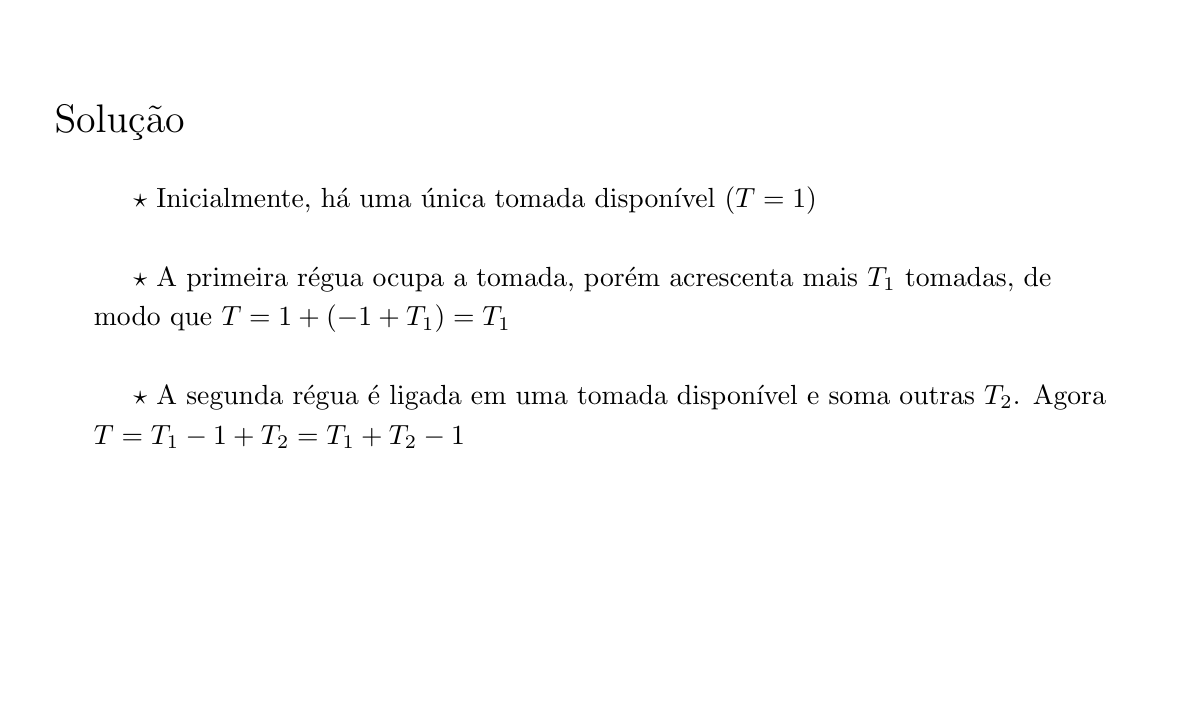
\begin{tikzpicture}
\node[draw,opacity=0] at (0, 0) {x};
\node[draw,opacity=0] at (14, 8) {x};

	\node[anchor=west] (title) at (0.0, 7.0) { \Large \bbbold{Solução} };


	\node[anchor=west] (a) at (1.0, 6.0) { $\star$ \bbtext{Inicialmente, há uma única tomada disponível $(T = 1)$} };


	\node[anchor=west] (b) at (1.0, 5.0) { $\star$ \bbtext{A primeira régua ocupa a tomada, porém acrescenta mais $T_1$ tomadas, de } };

	\node[anchor=west] (b1) at (0.5, 4.5) { \bbtext{modo que $T = 1 + (-1 + T_1) = T_1$} };


	\node[anchor=west] (c) at (1.0, 3.5) { $\star$ \bbtext{A segunda régua é ligada em uma tomada disponível e soma outras $T_2$. Agora} };

	\node[anchor=west] (c1) at (0.5, 3.0) { \bbtext{$T = T_1 - 1 + T_2 = T_1 + T_2 - 1$} };

\end{tikzpicture}
\end{frame}
\begin{frame}[plain,t]
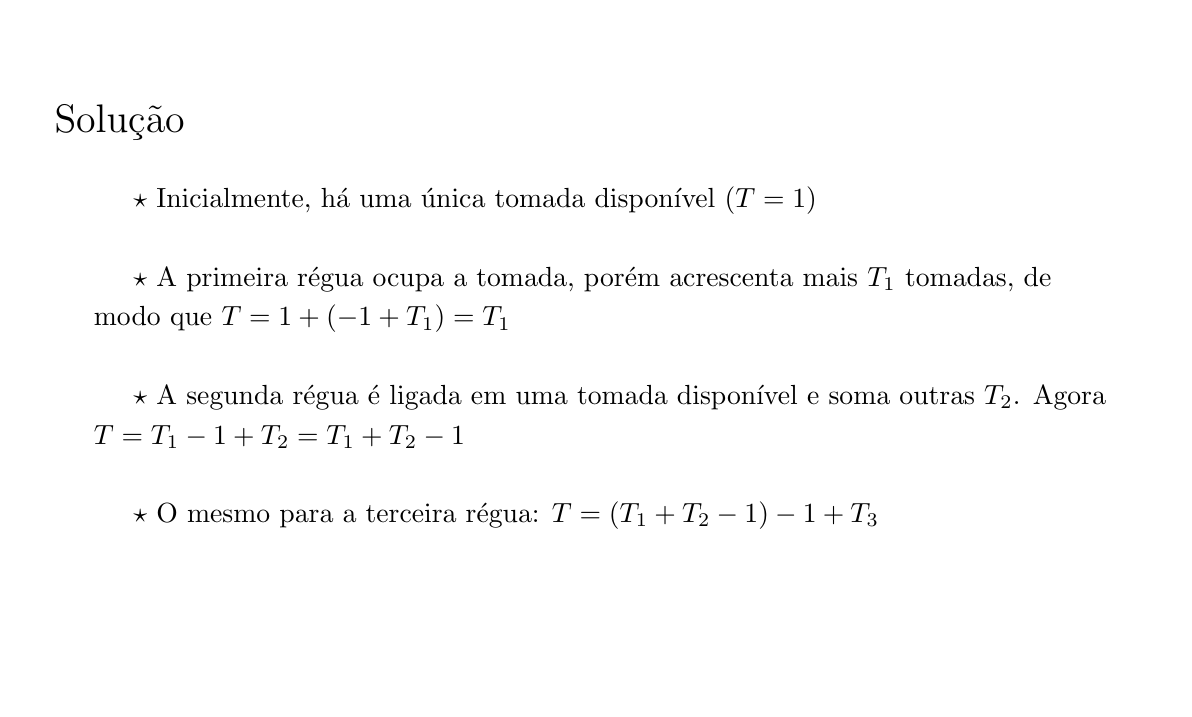
\begin{tikzpicture}
\node[draw,opacity=0] at (0, 0) {x};
\node[draw,opacity=0] at (14, 8) {x};

	\node[anchor=west] (title) at (0.0, 7.0) { \Large \bbbold{Solução} };


	\node[anchor=west] (a) at (1.0, 6.0) { $\star$ \bbtext{Inicialmente, há uma única tomada disponível $(T = 1)$} };


	\node[anchor=west] (b) at (1.0, 5.0) { $\star$ \bbtext{A primeira régua ocupa a tomada, porém acrescenta mais $T_1$ tomadas, de } };

	\node[anchor=west] (b1) at (0.5, 4.5) { \bbtext{modo que $T = 1 + (-1 + T_1) = T_1$} };


	\node[anchor=west] (c) at (1.0, 3.5) { $\star$ \bbtext{A segunda régua é ligada em uma tomada disponível e soma outras $T_2$. Agora} };

	\node[anchor=west] (c1) at (0.5, 3.0) { \bbtext{$T = T_1 - 1 + T_2 = T_1 + T_2 - 1$} };


	\node[anchor=west] (d) at (1.0, 2.0) { $\star$ \bbtext{O mesmo para a terceira régua: $T = (T_1 + T_2 - 1) - 1 + T_3$} };

\end{tikzpicture}
\end{frame}
\begin{frame}[plain,t]
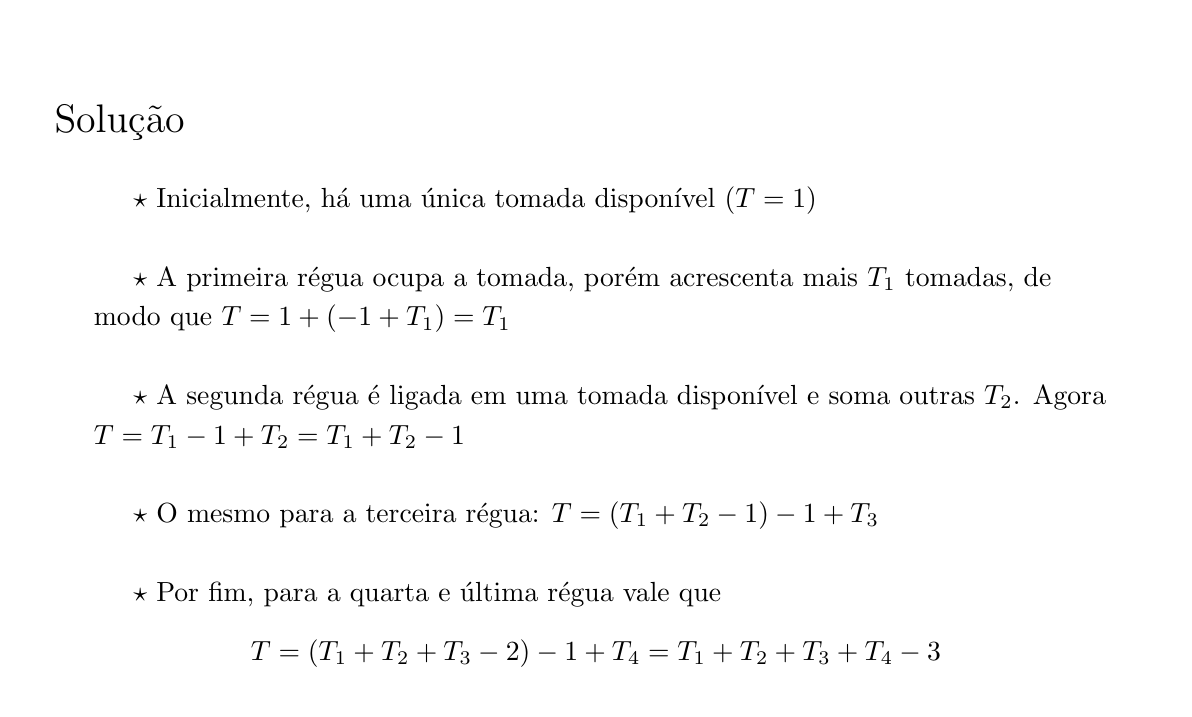
\begin{tikzpicture}
\node[draw,opacity=0] at (0, 0) {x};
\node[draw,opacity=0] at (14, 8) {x};

	\node[anchor=west] (title) at (0.0, 7.0) { \Large \bbbold{Solução} };


	\node[anchor=west] (a) at (1.0, 6.0) { $\star$ \bbtext{Inicialmente, há uma única tomada disponível $(T = 1)$} };


	\node[anchor=west] (b) at (1.0, 5.0) { $\star$ \bbtext{A primeira régua ocupa a tomada, porém acrescenta mais $T_1$ tomadas, de } };

	\node[anchor=west] (b1) at (0.5, 4.5) { \bbtext{modo que $T = 1 + (-1 + T_1) = T_1$} };


	\node[anchor=west] (c) at (1.0, 3.5) { $\star$ \bbtext{A segunda régua é ligada em uma tomada disponível e soma outras $T_2$. Agora} };

	\node[anchor=west] (c1) at (0.5, 3.0) { \bbtext{$T = T_1 - 1 + T_2 = T_1 + T_2 - 1$} };


	\node[anchor=west] (d) at (1.0, 2.0) { $\star$ \bbtext{O mesmo para a terceira régua: $T = (T_1 + T_2 - 1) - 1 + T_3$} };


	\node[anchor=west] (e) at (1.0, 1.0) { $\star$ \bbtext{Por fim, para a quarta e última régua vale que} };

	\node[] (e1) at (7.0, 0.25) { $T = (T_1 + T_2 + T_3 - 2) - 1 + T_4 = T_1 + T_2 + T_3 + T_4 - 3$ };

\end{tikzpicture}
\end{frame}
\begin{frame}[plain,t]
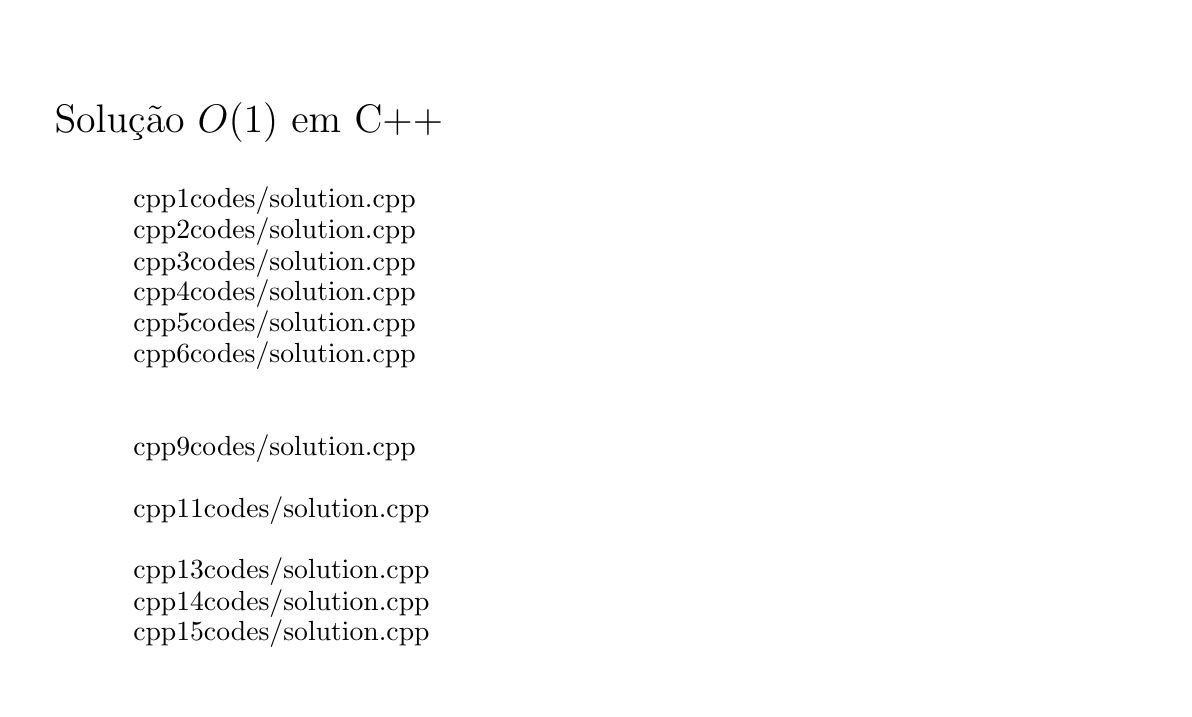
\begin{tikzpicture}
\node[draw,opacity=0] at (0, 0) {x};
\node[draw,opacity=0] at (14, 8) {x};

	\node[anchor=west] (title) at (0.0, 7.0) { \Large \bbbold{Solução $O(1)$ em C++} };

	\node[anchor=west] (line1) at (1.0, 6.0) { \inputline{cpp}{1}{codes/solution.cpp} };

	\node[anchor=west] (line2) at (1.0, 5.61) { \inputline{cpp}{2}{codes/solution.cpp} };

	\node[anchor=west] (line3) at (1.0, 5.21) { \inputline{cpp}{3}{codes/solution.cpp} };

	\node[anchor=west] (line4) at (1.0, 4.82) { \inputline{cpp}{4}{codes/solution.cpp} };

	\node[anchor=west] (line5) at (1.0, 4.43) { \inputline{cpp}{5}{codes/solution.cpp} };

	\node[anchor=west] (line6) at (1.0, 4.04) { \inputline{cpp}{6}{codes/solution.cpp} };



	\node[anchor=west] (line9) at (1.0, 2.86) { \inputline{cpp}{9}{codes/solution.cpp} };


	\node[anchor=west] (line11) at (1.0, 2.07) { \inputline{cpp}{11}{codes/solution.cpp} };


	\node[anchor=west] (line13) at (1.0, 1.29) { \inputline{cpp}{13}{codes/solution.cpp} };

	\node[anchor=west] (line14) at (1.0, 0.89) { \inputline{cpp}{14}{codes/solution.cpp} };

	\node[anchor=west] (line15) at (1.0, 0.5) { \inputline{cpp}{15}{codes/solution.cpp} };


\end{tikzpicture}
\end{frame}
\begin{frame}[plain,t]
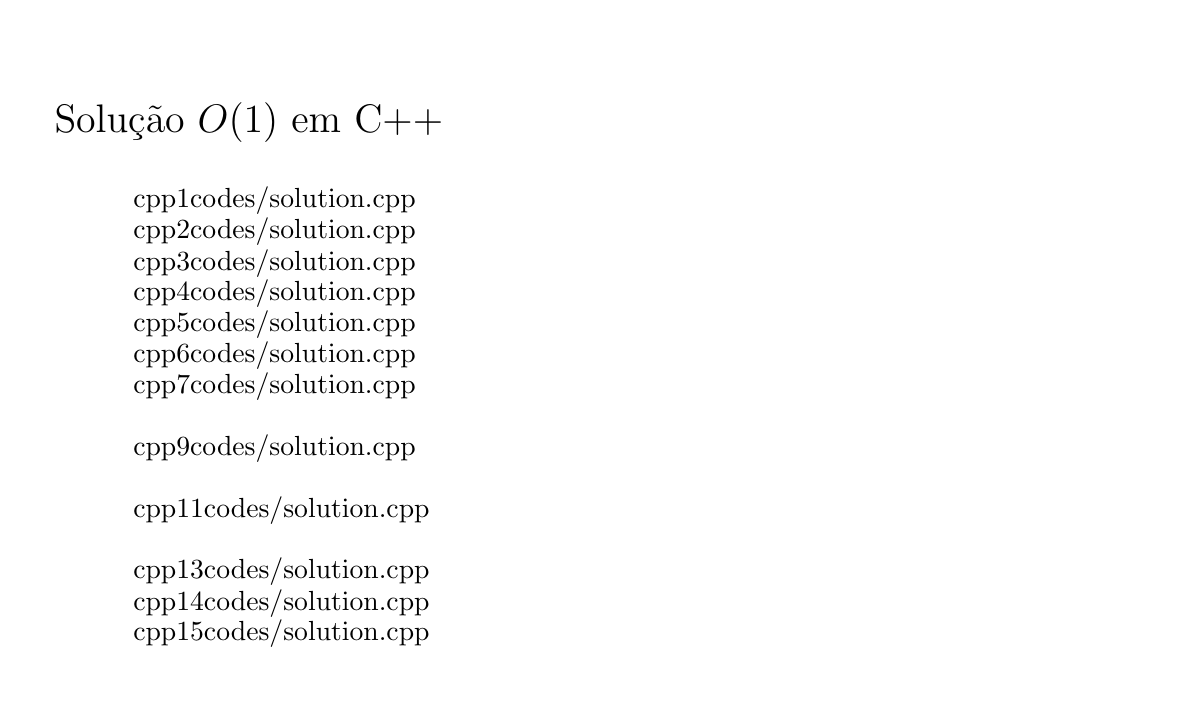
\begin{tikzpicture}
\node[draw,opacity=0] at (0, 0) {x};
\node[draw,opacity=0] at (14, 8) {x};

	\node[anchor=west] (title) at (0.0, 7.0) { \Large \bbbold{Solução $O(1)$ em C++} };

	\node[anchor=west] (line1) at (1.0, 6.0) { \inputline{cpp}{1}{codes/solution.cpp} };

	\node[anchor=west] (line2) at (1.0, 5.61) { \inputline{cpp}{2}{codes/solution.cpp} };

	\node[anchor=west] (line3) at (1.0, 5.21) { \inputline{cpp}{3}{codes/solution.cpp} };

	\node[anchor=west] (line4) at (1.0, 4.82) { \inputline{cpp}{4}{codes/solution.cpp} };

	\node[anchor=west] (line5) at (1.0, 4.43) { \inputline{cpp}{5}{codes/solution.cpp} };

	\node[anchor=west] (line6) at (1.0, 4.04) { \inputline{cpp}{6}{codes/solution.cpp} };

	\node[anchor=west] (line7) at (1.0, 3.64) { \inputline{cpp}{7}{codes/solution.cpp} };


	\node[anchor=west] (line9) at (1.0, 2.86) { \inputline{cpp}{9}{codes/solution.cpp} };


	\node[anchor=west] (line11) at (1.0, 2.07) { \inputline{cpp}{11}{codes/solution.cpp} };


	\node[anchor=west] (line13) at (1.0, 1.29) { \inputline{cpp}{13}{codes/solution.cpp} };

	\node[anchor=west] (line14) at (1.0, 0.89) { \inputline{cpp}{14}{codes/solution.cpp} };

	\node[anchor=west] (line15) at (1.0, 0.5) { \inputline{cpp}{15}{codes/solution.cpp} };



\end{tikzpicture}
\end{frame}
\begin{frame}[plain,t]
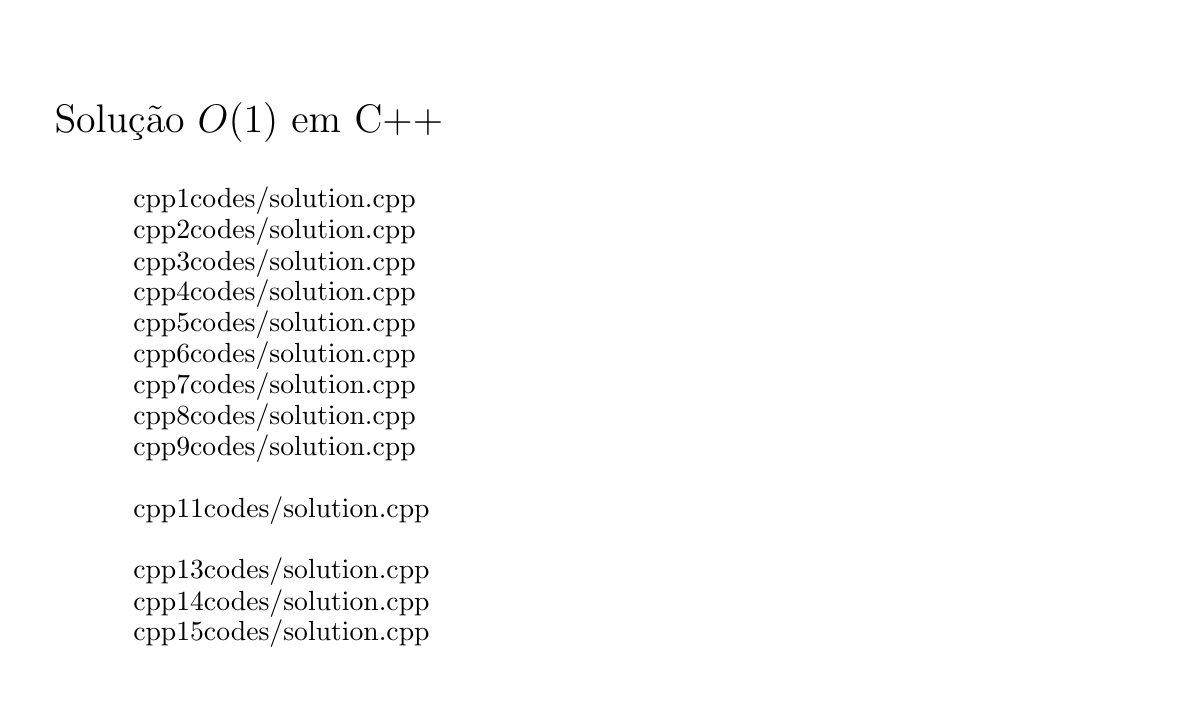
\begin{tikzpicture}
\node[draw,opacity=0] at (0, 0) {x};
\node[draw,opacity=0] at (14, 8) {x};

	\node[anchor=west] (title) at (0.0, 7.0) { \Large \bbbold{Solução $O(1)$ em C++} };

	\node[anchor=west] (line1) at (1.0, 6.0) { \inputline{cpp}{1}{codes/solution.cpp} };

	\node[anchor=west] (line2) at (1.0, 5.61) { \inputline{cpp}{2}{codes/solution.cpp} };

	\node[anchor=west] (line3) at (1.0, 5.21) { \inputline{cpp}{3}{codes/solution.cpp} };

	\node[anchor=west] (line4) at (1.0, 4.82) { \inputline{cpp}{4}{codes/solution.cpp} };

	\node[anchor=west] (line5) at (1.0, 4.43) { \inputline{cpp}{5}{codes/solution.cpp} };

	\node[anchor=west] (line6) at (1.0, 4.04) { \inputline{cpp}{6}{codes/solution.cpp} };

	\node[anchor=west] (line7) at (1.0, 3.64) { \inputline{cpp}{7}{codes/solution.cpp} };

	\node[anchor=west] (line8) at (1.0, 3.25) { \inputline{cpp}{8}{codes/solution.cpp} };

	\node[anchor=west] (line9) at (1.0, 2.86) { \inputline{cpp}{9}{codes/solution.cpp} };


	\node[anchor=west] (line11) at (1.0, 2.07) { \inputline{cpp}{11}{codes/solution.cpp} };


	\node[anchor=west] (line13) at (1.0, 1.29) { \inputline{cpp}{13}{codes/solution.cpp} };

	\node[anchor=west] (line14) at (1.0, 0.89) { \inputline{cpp}{14}{codes/solution.cpp} };

	\node[anchor=west] (line15) at (1.0, 0.5) { \inputline{cpp}{15}{codes/solution.cpp} };




\end{tikzpicture}
\end{frame}
\begin{frame}[plain,t]
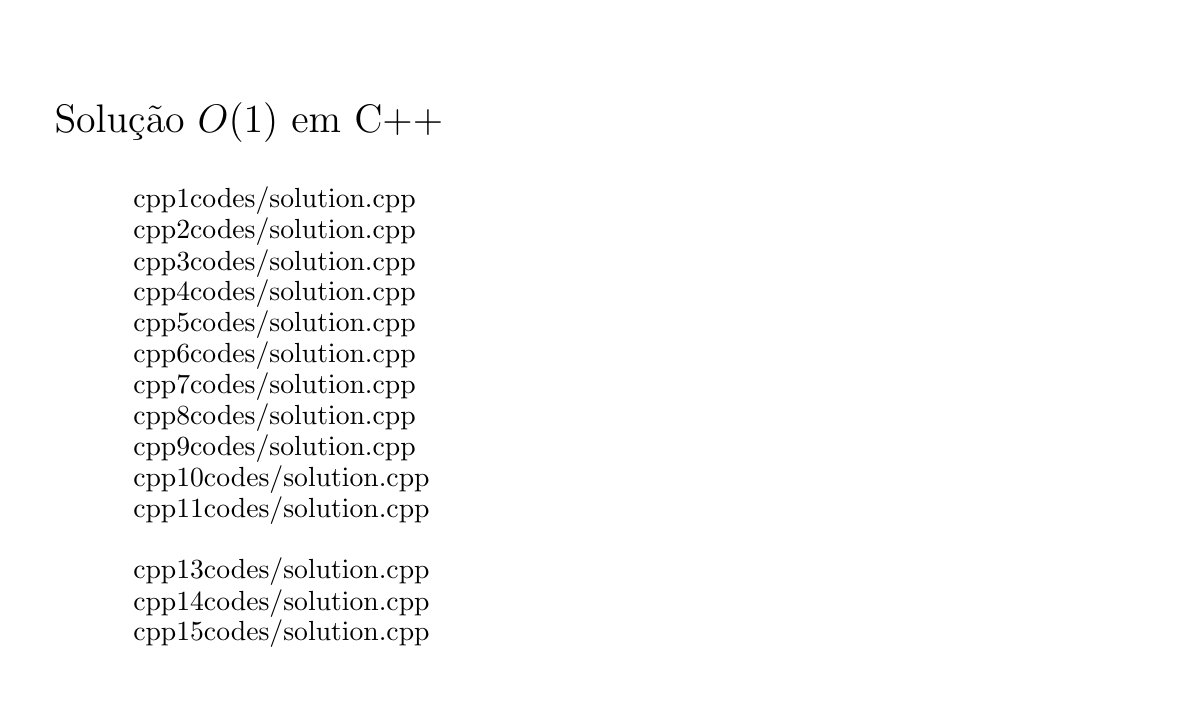
\begin{tikzpicture}
\node[draw,opacity=0] at (0, 0) {x};
\node[draw,opacity=0] at (14, 8) {x};

	\node[anchor=west] (title) at (0.0, 7.0) { \Large \bbbold{Solução $O(1)$ em C++} };

	\node[anchor=west] (line1) at (1.0, 6.0) { \inputline{cpp}{1}{codes/solution.cpp} };

	\node[anchor=west] (line2) at (1.0, 5.61) { \inputline{cpp}{2}{codes/solution.cpp} };

	\node[anchor=west] (line3) at (1.0, 5.21) { \inputline{cpp}{3}{codes/solution.cpp} };

	\node[anchor=west] (line4) at (1.0, 4.82) { \inputline{cpp}{4}{codes/solution.cpp} };

	\node[anchor=west] (line5) at (1.0, 4.43) { \inputline{cpp}{5}{codes/solution.cpp} };

	\node[anchor=west] (line6) at (1.0, 4.04) { \inputline{cpp}{6}{codes/solution.cpp} };

	\node[anchor=west] (line7) at (1.0, 3.64) { \inputline{cpp}{7}{codes/solution.cpp} };

	\node[anchor=west] (line8) at (1.0, 3.25) { \inputline{cpp}{8}{codes/solution.cpp} };

	\node[anchor=west] (line9) at (1.0, 2.86) { \inputline{cpp}{9}{codes/solution.cpp} };

	\node[anchor=west] (line10) at (1.0, 2.46) { \inputline{cpp}{10}{codes/solution.cpp} };

	\node[anchor=west] (line11) at (1.0, 2.07) { \inputline{cpp}{11}{codes/solution.cpp} };


	\node[anchor=west] (line13) at (1.0, 1.29) { \inputline{cpp}{13}{codes/solution.cpp} };

	\node[anchor=west] (line14) at (1.0, 0.89) { \inputline{cpp}{14}{codes/solution.cpp} };

	\node[anchor=west] (line15) at (1.0, 0.5) { \inputline{cpp}{15}{codes/solution.cpp} };





\end{tikzpicture}
\end{frame}
\begin{frame}[plain,t]
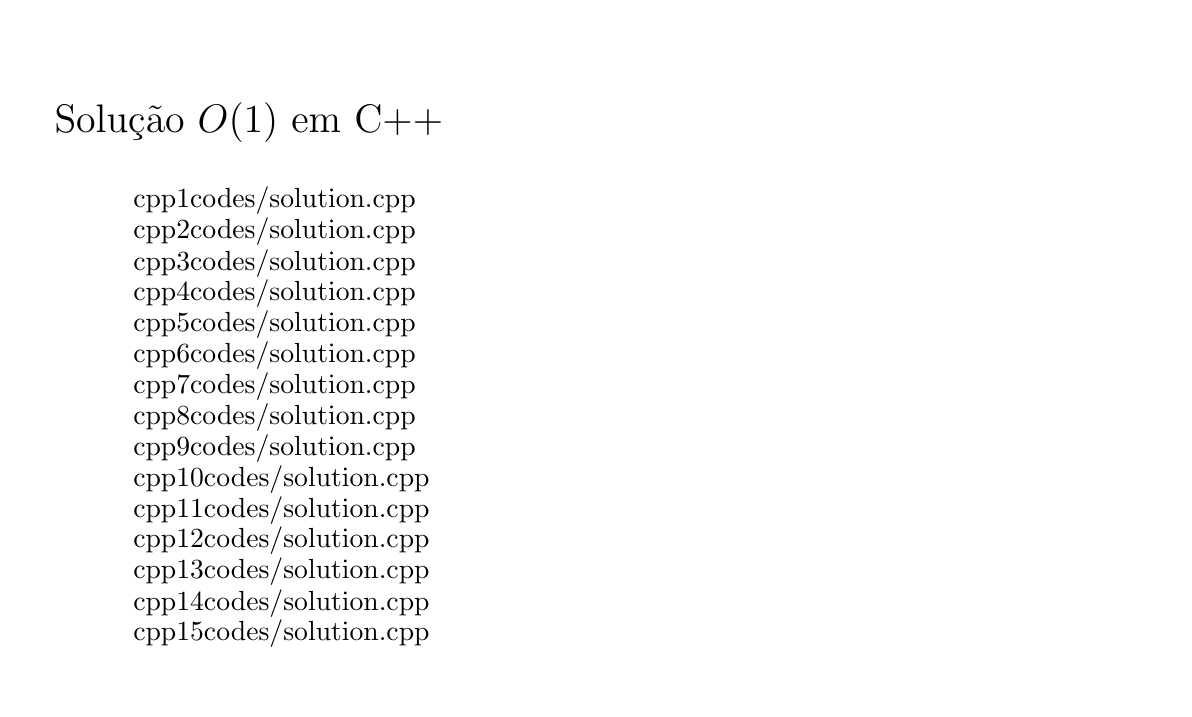
\begin{tikzpicture}
\node[draw,opacity=0] at (0, 0) {x};
\node[draw,opacity=0] at (14, 8) {x};

	\node[anchor=west] (title) at (0.0, 7.0) { \Large \bbbold{Solução $O(1)$ em C++} };

	\node[anchor=west] (line1) at (1.0, 6.0) { \inputline{cpp}{1}{codes/solution.cpp} };

	\node[anchor=west] (line2) at (1.0, 5.61) { \inputline{cpp}{2}{codes/solution.cpp} };

	\node[anchor=west] (line3) at (1.0, 5.21) { \inputline{cpp}{3}{codes/solution.cpp} };

	\node[anchor=west] (line4) at (1.0, 4.82) { \inputline{cpp}{4}{codes/solution.cpp} };

	\node[anchor=west] (line5) at (1.0, 4.43) { \inputline{cpp}{5}{codes/solution.cpp} };

	\node[anchor=west] (line6) at (1.0, 4.04) { \inputline{cpp}{6}{codes/solution.cpp} };

	\node[anchor=west] (line7) at (1.0, 3.64) { \inputline{cpp}{7}{codes/solution.cpp} };

	\node[anchor=west] (line8) at (1.0, 3.25) { \inputline{cpp}{8}{codes/solution.cpp} };

	\node[anchor=west] (line9) at (1.0, 2.86) { \inputline{cpp}{9}{codes/solution.cpp} };

	\node[anchor=west] (line10) at (1.0, 2.46) { \inputline{cpp}{10}{codes/solution.cpp} };

	\node[anchor=west] (line11) at (1.0, 2.07) { \inputline{cpp}{11}{codes/solution.cpp} };

	\node[anchor=west] (line12) at (1.0, 1.68) { \inputline{cpp}{12}{codes/solution.cpp} };

	\node[anchor=west] (line13) at (1.0, 1.29) { \inputline{cpp}{13}{codes/solution.cpp} };

	\node[anchor=west] (line14) at (1.0, 0.89) { \inputline{cpp}{14}{codes/solution.cpp} };

	\node[anchor=west] (line15) at (1.0, 0.5) { \inputline{cpp}{15}{codes/solution.cpp} };






\end{tikzpicture}
\end{frame}
\end{document}
